\index{general}{Essential Boundary Conditions}
\index{general}{Natural Boundary Conditions}
\begin{flushright} {\tiny {\color{gray} kinematic\_bc.tex}} \end{flushright}


\begin{center}
\includegraphics[width=8cm]{images/boundary_conditions/bc1}
\end{center}


\begin{center}
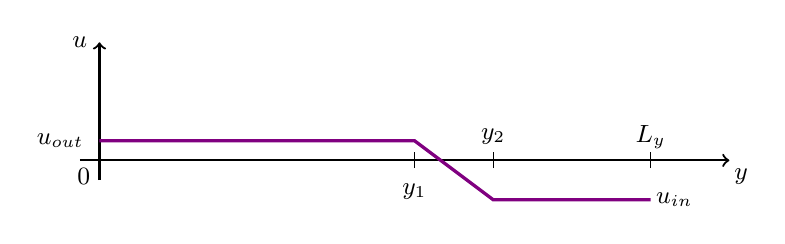
\begin{tikzpicture}
%\draw[fill=gray!23,gray!23](0,0) rectangle (10,3);
%\draw[step=0.5cm,gray,very thin] (0,0) grid (10,3); %background grid
\draw[thick,->] (0.75,1) -- (9,1)  ; 
\draw[thick,->] (1,0.75) -- (1,2.5)  ; 
\draw[-] (5,0.9) -- (5,1.1)  ; 
\draw[-] (6,0.9) -- (6,1.1)  ; 
\draw[-] (8,0.9) -- (8,1.1)  ; 
\draw[very thick, violet] (1,1.25)--(5,1.25) -- (6,0.5) -- (8,0.5) ; 
\node[] at (0.8,0.8) {\small $0$};
\node[] at (9.15,0.8) {\small $y$};
\node[] at (5,0.6) {\small $y_1$};
\node[] at (6,1.3) {\small $y_2$};
\node[] at (8,1.3) {\small $L_y$};
\node[] at (8.3,0.5) {\small $u_{in}$};
\node[] at (0.5,1.25) {\small $u_{out}$};
\node[] at (0.75,2.5) {\small $u$};
\end{tikzpicture}
\end{center}



The velocity on the side is given by
\begin{eqnarray}
u(y) &=& u_{out} \quad\quad y<y_1 \nn\\
u(y) &=& \frac{u_{in}-u_{out}}{y_2-y_1}(y-y_1) + u_{out} \quad\quad y_1<y<y_2 \nn\\
u(y) &=& u_{in} \quad\quad y>y_2 \nn
\end{eqnarray}
Note that $u_{in}$ and $u_{out}$ can be positive or negative, but 
of opposite signs.
The requirement for volume conservation is:
\[
\Phi=\int_{0}^{L_y} u(y) dy = 0
\]
Having chosen $u_{in}$ (the velocity of the plate), one can then compute $v_{out}$
as a function of $y_1$ and $y_2$.

\begin{eqnarray}
\Phi
&=&
\underbrace{\int_{0}^{y_1} u(y) dy}_{\Phi_1}  +
\underbrace{\int_{y_1}^{y_2} u(y) dy }_{\Phi_2}  +
\underbrace{\int_{y_2}^{L_y} u(y) dy }_{\Phi_3}\nn
\end{eqnarray}
with
\begin{eqnarray}
\Phi_1 &=& u_{out} y_1 \nn\\
\Phi_2 
&=& \int_{y_1}^{y_2} u(y) dy \nn\\
&=& \int_{y_1}^{y_2} \left[ \frac{u_{in}-u_{out}}{y_2-y_1}(y-y_1) + u_{out}   \right] dy \nn\\
&=& \int_{y_1}^{y_2} \frac{u_{in}-u_{out}}{y_2-y_1}(y-y_1)  dy  +   \int_{y_1}^{y_2}  u_{out} dy \nn\\
&=& \frac{u_{in}-u_{out}}{y_2-y_1} \int_{y_1}^{y_2} (y-y_1)  dy  +   (y_2-y_1) u_{out}  \nn\\
&=& \frac{u_{in}-u_{out}}{y_2-y_1} \left[ \frac12 y^2 - y_1y   \right]_{y_1}^{y_2} +   (y_2-y_1) u_{out}  \nn\\
&=& \frac{u_{in}-u_{out}}{y_2-y_1} ( \frac12 y_2^2 - y_1y_2 - \frac12y_1^2 + y_1^2 ) +   (y_2-y_1) u_{out}  \nn\\
&=& \frac{u_{in}-u_{out}}{y_2-y_1} \frac12 ( y_2^2 - 2y_1y_2 + y_1^2 ) +   (y_2-y_1) u_{out}  \nn\\
&=& \frac{u_{in}-u_{out}}{y_2-y_1} \frac12 ( y_2-y_1 )^2 +   (y_2-y_1) u_{out}  \nn\\
&=& (u_{in}-u_{out}) \frac12 ( y_2-y_1 ) +   (y_2-y_1) u_{out}  \nn\\
&=& \frac{1}{2}(u_{in}+u_{out})(y_2-y_1)  \nn\\
\Phi_3 &=& (L_y-y_2) u_{in} \nn
\end{eqnarray}
so that in the end
\begin{eqnarray}
\Phi &=& \Phi_1+\Phi_2+\Phi_3 \nn\\
&=& u_{out} [y_1 + \frac{1}{2}(y_2-y_1) ] + u_{in} [ \frac{1}{2}(y_2-y_1)  + (L_y-y_2) ] \nn\\
&=& u_{out}\frac{1}{2} (y_1 + y_2 ) + u_{in} [ L_y - \frac{1}{2}(y_1+y_2) ] \nn
\end{eqnarray}
and finally, solving for $u_{out}$
\begin{mdframed}[backgroundcolor=blue!5]
\[
u_{out} = -u_{in} \frac{ L_y - \frac{1}{2}(y_1+y_2)}{ \frac{1}{2} (y_1 + y_2 ) }
\]
\end{mdframed}


In some cases one may wish to prescribe a zero velocity 
below the 660 discontinuity (given by $y=y_1$) on the following 
figure:

\begin{center}
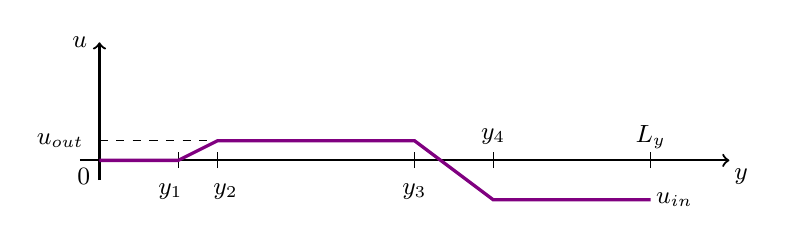
\begin{tikzpicture}
%\draw[fill=gray!23,gray!23](0,0) rectangle (10,3);
%\draw[step=0.5cm,gray,very thin] (0,0) grid (10,3); %background grid
\draw[thick,->] (0.75,1) -- (9,1)  ; 
\draw[thick,->] (1,0.75) -- (1,2.5)  ; 
\draw[-] (2,0.9) -- (2,1.1)  ; 
\draw[-] (2.5,0.9) -- (2.5,1.1)  ; 
\draw[-] (5,0.9) -- (5,1.1)  ; 
\draw[-] (6,0.9) -- (6,1.1)  ; 
\draw[-] (8,0.9) -- (8,1.1)  ; 
\draw[thin, dashed] (1,1.25) -- (2.5,1.25)  ; 
\draw[very thick, violet] (1,1)--(2,1)--(2.5,1.25)--(5,1.25) -- (6,0.5) -- (8,0.5) ; 
\node[] at (0.8,0.8) {\small $0$};
\node[] at (9.15,0.8) {\small $y$};
\node[] at (1.9,0.6) {\small $y_1$};
\node[] at (2.6,0.6) {\small $y_2$};
\node[] at (5,0.6) {\small $y_3$};
\node[] at (6,1.3) {\small $y_4$};
\node[] at (8,1.3) {\small $L_y$};
\node[] at (8.3,0.5) {\small $u_{in}$};
\node[] at (0.5,1.25) {\small $u_{out}$};
\node[] at (0.75,2.5) {\small $u$};
\end{tikzpicture}
\end{center}

